\documentclass[12pt]{article}
\usepackage[fleqn]{amsmath}
\usepackage{amssymb}
\usepackage{amsthm}
\usepackage{amssymb}
\usepackage{tikz}
\usepackage{pgfplots}
    \pgfplotsset{width=10cm,compat=1.9}
\usepackage{tipa}
\usepackage{hyperref}
\usepackage{mathtools}
    \hypersetup{colorlinks=true,citecolor=blue,urlcolor =black,linkbordercolor={1 0 0}}
\newcommand*\circled[1]{\tikz[baseline=(char.base)]{
    \node[shape=circle,draw,inner sep=2pt] (char) {#1};}}
\newcommand{\BR}{\mathbb R}
\newcommand{\BN}{\mathbb N}
\newcommand{\prm}{^\prime}
\newcommand{\doubleprime}{^{\prime\prime}}
\newcommand{\phii}{\varphi}
\title{Lecture 23}
\begin{document}
\maketitle
\vspace*{-0.25in}
\begin{center}
	Anders Sundheim \\
	\href{mailto:asundheim@wisc.edu}{{\tt asundheim@wisc.edu}}
\end{center}
\section*{Change of variables in a multiple integral}

    \[ \int_Sf(x)\,dx=\idotsint\limits_S f(x_1,x_2,\dots,x_n)\,dx_1\,dx_2\,\dots\,dx_n:S\subset\BR^n \]
    \[
      \begin{cases}
          x_1=X_1(u_1,u_2,\dots,u_n) \\
          x_2=X_2(u_1,u_2,\dots,u_n) \\
          \vdots \\
          x_n=X_n(u_1,u_2,\dots,u_n)
      \end{cases}
      \Rightarrow (u_1,\dots,u_n)\mapsto(x_1,\dots,x_n), u\mapsto x
    \]
    \[ 
        x=X(u):
        \begin{cases}
            X(u)\text{ continuous and differentiable} \\
            u\mapsto X(u)=x \text{ is one-to-one}
        \end{cases}
    \]
    Jacobian Matrix \\
    \[
        DX(u)=
        \begin{pmatrix*}
            \frac{dX_1}{du_1} & \dots & \frac{dX_1}{du_n} \\
            \vdots & & \vdots \\
            \frac{dX_n}{du_1} & \dots & \frac{dX_n}{du_n}
        \end{pmatrix*}
    \]
    Jacobian determinant: $J(u)=\text{det}[DX(u)]\neq 0$ \\
    \newline \newline \newline \\
    \[ \int_Sf(x)\,dx \quad S=X(T) \]
    \[
        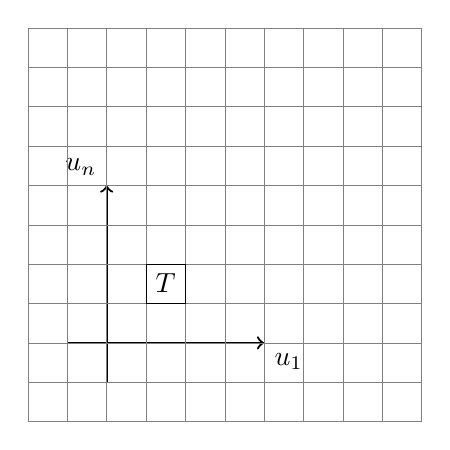
\begin{tikzpicture}[scale=0.5]
            \draw[thick,->] (-1,0) -- (4,0) node[anchor=north west] {$u_1$};
            \draw[thick,->] (0,-1) -- (0,4) node[anchor=south east] {$u_n$};
            \draw[step=1cm,gray,very thin] (-2,-2) grid (8,8);
            \draw (1, 1) rectangle (2,2);
            \draw (1.5,2) node[anchor=north]{$T$};
        \end{tikzpicture}
        \xrightarrow{x=X(u)}
        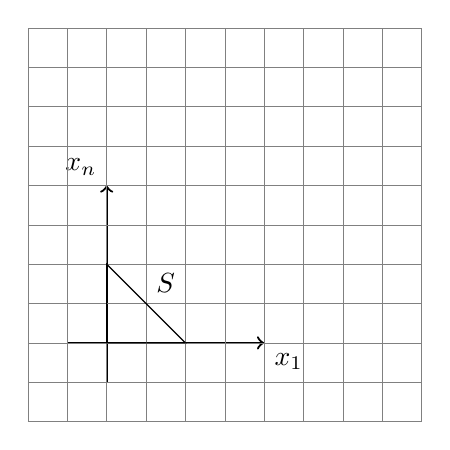
\begin{tikzpicture}[scale=0.5]
            \draw[thick,->] (-1,0) -- (4,0) node[anchor=north west] {$x_1$};
            \draw[thick,->] (0,-1) -- (0,4) node[anchor=south east] {$x_n$};
            \draw[step=1cm,gray,very thin] (-2,-2) grid (8,8);
            \draw (0, 0) -- (0,2) -- (2,0) -- cycle;
            \draw (1.5,2) node[anchor=north]{$S$};
        \end{tikzpicture}
    \]
    \[ \int_Sf(x)\,dx=\int_Tf(X(u))|J(u)|\,du \]
\section*{Cylindrical coordinates $\BR^3\{x,y,z\}$}
    \[
        \begin{cases}
            x=r\cos\theta \\
            y=r\sin\theta \\
            z=z
        \end{cases}
        \Rightarrow (r,\theta,z)\mapsto(x,y,z):
        \begin{cases}
            0<r<+\infty \\
            0\leq\theta\leq 2\pi \\
            z\in\BR
        \end{cases}
    \]
    \[
        J(r,\theta,z)=
        \begin{vmatrix*}
            \frac{dx}{dr} & \frac{dx}{d\theta} & \frac{dx}{dz} \\
            \frac{dy}{dr} & \frac{dy}{d\theta} & \frac{dy}{dz} \\
            \frac{dz}{dr} & \frac{dz}{d\theta} & \frac{dz}{dz}
        \end{vmatrix*}
        =
        \begin{vmatrix*}
            \cos\theta & -r\sin\theta & 0 \\
            \sin\theta & r\cos\theta & 0 \\
            0 & 0 & 1
        \end{vmatrix*}
        = r
    \]
    \[ \iiint_Sf(x,y,z)\,dx\,dy\,dz=\iiint_T(r\cos\theta,r\sin\theta,z)r\,dr\,d\theta\,dz \]
    \subsection*{Example}
        Cylinder of radius $R$ and height $H$ \\
        \[
            \begin{cases}
                0<r<R \\
                0\leq\theta\leq 2\pi \\
                0\leq z\leq H  
            \end{cases}
            \Rightarrow \iiint_Tf=\int_0^H\int_0^{2\pi}\int_0^Rf
        \]
\section*{Spherical Coordinates in $\BR^3\{x,y,z\}$}
    \[
        \begin{cases}
            x=\rho\sin\phii\cos\theta \\
            y=\rho\sin\phii\sin\theta \\
            z=\rho\cos\phii
        \end{cases}
        \Rightarrow (\rho,\phii,\theta)\mapsto(x,y,z):
        \begin{cases}
            0<\rho<+\infty \\
            0<\phii<\pi \\
            0\leq\theta<2\pi
        \end{cases}
    \]
    $r=\rho\sin\phii$ \\
    \[
        J(\rho,\phii,\theta)=
        \begin{vmatrix*}
            \frac{dx}{d\rho} & \frac{dx}{d\phii} & \frac{dx}{d\theta} \\
            \frac{dy}{d\rho} & \frac{dy}{d\phii} & \frac{dy}{d\theta} \\
            \frac{dz}{d\rho} & \frac{dz}{d\phii} & \frac{dz}{d\theta}
        \end{vmatrix*}
        =
        \begin{vmatrix*}
            \sin\phii\cos\theta & \rho\cos\phii\cos\theta & -\rho\sin\phii\sin\theta \\
            \sin\phii\sin\theta & \rho\cos\phii\sin\theta & \rho\sin\phii\cos\theta \\
            \cos\phii & -\rho\sin\phii & 0
        \end{vmatrix*}
        = \rho^2\sin\phii   
    \]
    \[ \iiint_Sf(x,y,z)\,dx\,dy\,dz=\iiint_Tf(\rho\sin\phii\cos\theta,\rho\sin\phii\sin\theta,\rho\sin\phii)\rho^2\sin\phii\,d\rho\,d\phii\,d\theta \]
\end{document}
